\chapter{\IfLanguageName{dutch}{Stand van zaken}{State of the art}}
\label{ch:stand-van-zaken}

% Tip: Begin elk hoofdstuk met een paragraaf inleiding die beschrijft hoe
% dit hoofdstuk past binnen het geheel van de bachelorproef. Geef in het
% bijzonder aan wat de link is met het vorige en volgende hoofdstuk.

% Pas na deze inleidende paragraaf komt de eerste sectiehoofding.

In de inleiding is duidelijk geworden dat het onderzoek gericht zal zijn op twee mogelijke dataformaten aan de hand van 2 verschillende structuren, namelijk JSON aan de hand van REST en gRPC aan de hand van Protocol Buffers. Om dit onderzoek volledig te kunnen begrijpen is het belangrijk om de werking en de basisprincipes van deze dataformaten en de daarbij behorende structuren te begrijpen. Om deze reden zullen eerst de werking en basisprincipes van JSON en RESTful API worden uitgelegd, en als volgt die van gRPC en Protocol Buffers.

\section{JSON}
\label{sec:JSON}

\subsection{Algemeen}
\label{subsec:Algemeen}

JSON is een dataformaat zoals bijvoorbeeld XML en de afkorting staat voor JavaScript Object Notation. JSON is zoals beschreven in Standard ECMA-404 ~\autocite{Json2017} een dataformaat dat geïnspireerd is door de object constanten van JavaScript dat ook gekend staat als ECMAScript en is een structuur van accolades, haakjes, dubbele punten en komma's die zeer nuttig kunnen zijn in verschillende contexten, profielen en applicaties. Een voorbeeld hiervan is te zien in figuur \ref{fig:jsonExample}.

\begin{figure}[H]
    \centering
    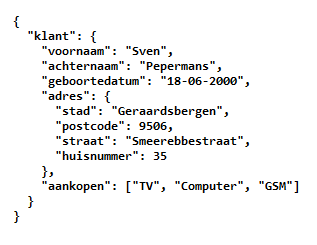
\includegraphics[scale=1.50]{jsonExample}
    \caption[JSON Example]{Een voorbeeld van een JSON.}
    \label{fig:jsonExample}
\end{figure}

JSON mag niet gezien worden als een specificatie van een gegevensuitwisseling want dat is het ook niet. Bij een zinvolle gegevensuitwisseling wordt er een overeenstemming over de structuur die gekoppeld is aan een gebruik van JSON tussen producent en consument vereist. JSON kan wel gezien worden als een syntactisch raamwerk waaraan een specifieke structuur kan worden gekoppeld.

Doordat er veel verschillende types getallen zijn zoals decimale en binaire getallen, kiest JSON enkel voor een weergave van getallen die mensen gebruiken, namelijk een reeks cijfers. Ook al zijn alle programmeertalen het niet altijd eens over de interne representaties van getallen, ze weten wel hoe ze cijferreeksen moeten begrijpen.

 Objecten kunnen op veel verschillende manieren voorgesteld worden, met andere woorden kunnen de modellen van objecten heel erg uiteenlopen. Om dit probleem aan te pakken biedt JSON een eenvoudige notatie aan voor het uitdrukken van verzamelingen met naam / waarde-paren. Om zulke verzamelingen weer te geven hebben de meeste programmeertalen reeds een functie zoals struct, map, hash en object.
Daarnaast biedt JSON ook ondersteuning voor geordende zoeklijsten, alsook hiervoor hebben alle programmeertalen een functie om deze weer te geven zoals array, vector en list. Aangezien objecten en arrays zich kunnen nesten, kunnen aan de hand van JSON complexe structuren zoals boomstructuren worden gerepresenteerd.

Hieruit kan worden geconcludeerd dat door het aanvaarden van JSON's simpele conventies, complexe datastructuren uitgewisseld kunnen worden tussen wat anders incompatiebele programmeertalen zijn.



\subsection{JSON in detail bekeken}
\label{subsec:JSON in detail bekeken}

Een JSON-tekst bestaat uit een reeks tokens die gevormd zijn uit Unicode-codepunten en die in overeenstemming zijn met de achterliggende JSON grammatica. Zo een reeks tokens bevat tekenreeksen, cijfers, zes structurele tokens en drie letterlijke naamtokens.
Hieronder volgt een opsomming van de zes structurele tokens en de drie literal name tokens.

De zes structurele tokens:

\begin{itemize}
    \item $\rbrack$ Linker vierkante haak
    \item $\rbrack$ Rechter vierkante haak
    \item \{ Linker accolade
    \item \} Rechter accolade
    \item : Dubbele punt
    \item , Komma
\end{itemize}

De drie literal name tokens:

\begin{itemize}
    \item true  
    \item false     
    \item null      
\end{itemize}

Voor of na de meeste tokens is het toegestaan om witruimte te gebruiken, echter niet in ze allemaal, een spatie is hierop een uitzondering en is wel toegestaan in strings. deze witruimte kan beschreven worden als een willekeurige reeks van één of meerdere van onderstaande codepunten.

\begin{itemize}
    \item Tekentabel       
    \item Regelinvoer       
    \item Regelterugloop   
    \item Spatie           
\end{itemize}


\subsection{Waarden}
\label{subsec:Waarden}

De bovengestelde tokens vormen de ruggengraat van een JSON-bestand, echter is het de bedoeling dat een JSON-bestand data overdraagt. Deze data kan aan de hand van verschillende waarden worden voorgesteld, namelijk als objecten, arrays, nummers, strings, true, false en null. Alle mogelijke waarden zijn zichtbaar in figuur \ref{jsonValue}.

\begin{figure}[ht]
    \centering
    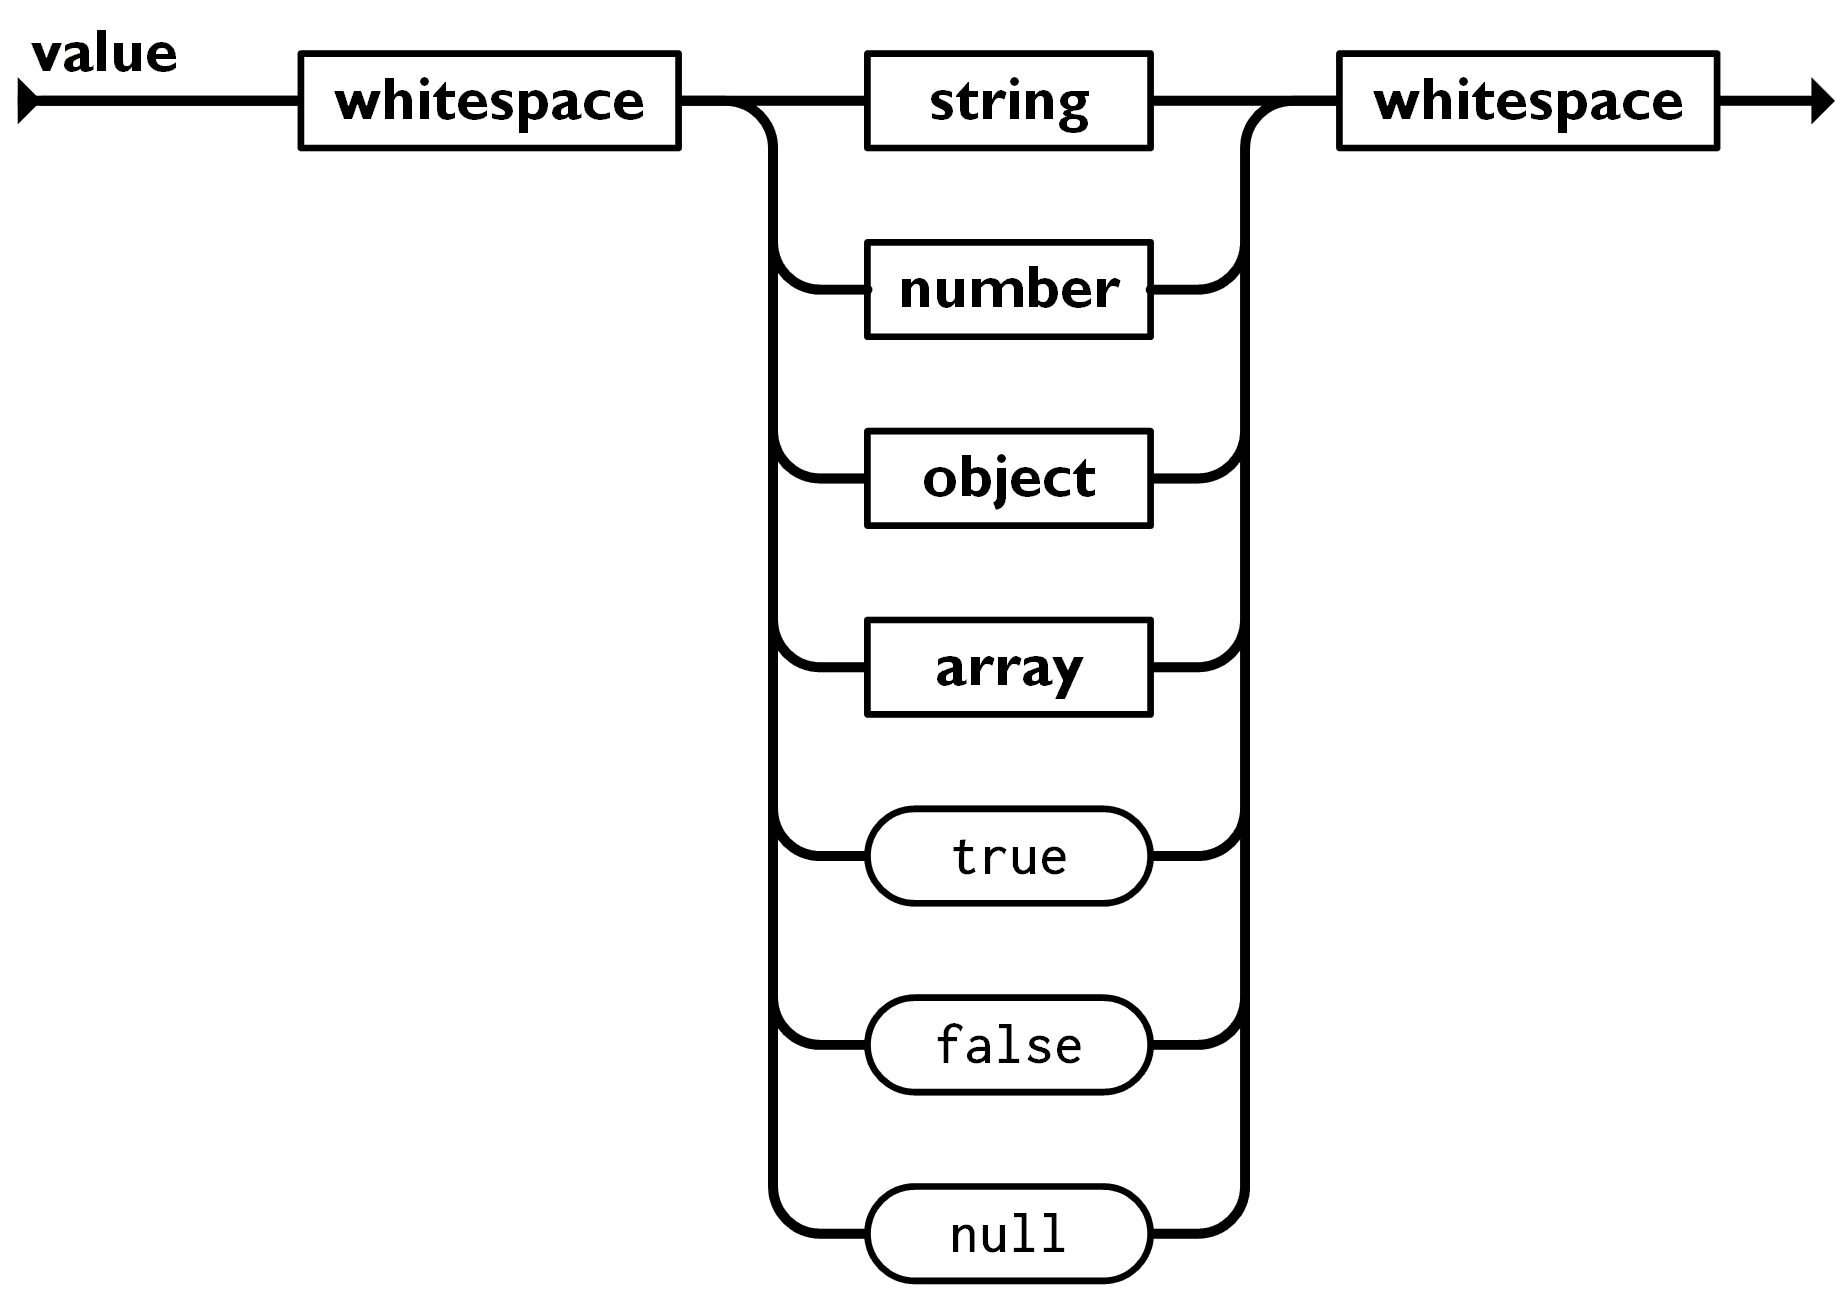
\includegraphics[scale=0.75]{jsonValue}
   \caption[JSON values]{De structuur van een JSON-waarde met alle mogelijke waarden die deze kan bevatten. Bron: \url{www.json.org}}
   \label{fig:jsonValue}
\end{figure}

De eerste waarden die besproken worden zijn de objecten, deze worden voorgesteld door een paar accolades die geen of meerdere name/value paren kunnen omringen zoals te zien is in figuur \ref{fig:jsonObject} en in figuur \ref{fig:objectEx}. In zo een name/value paar is de naam een string en wordt gevolgd door een dubbele punt die de naam en waarde van elkaar onderscheidt. 
Na de waarde kan optioneel een komma gezet worden, deze onderscheidt de waarde en de volgende naam van elkaar. Tot slot moeten de namen niet uniek zijn en moeten ze geen bepaalde ordening volgen.

\begin{figure}[H]
    \centering
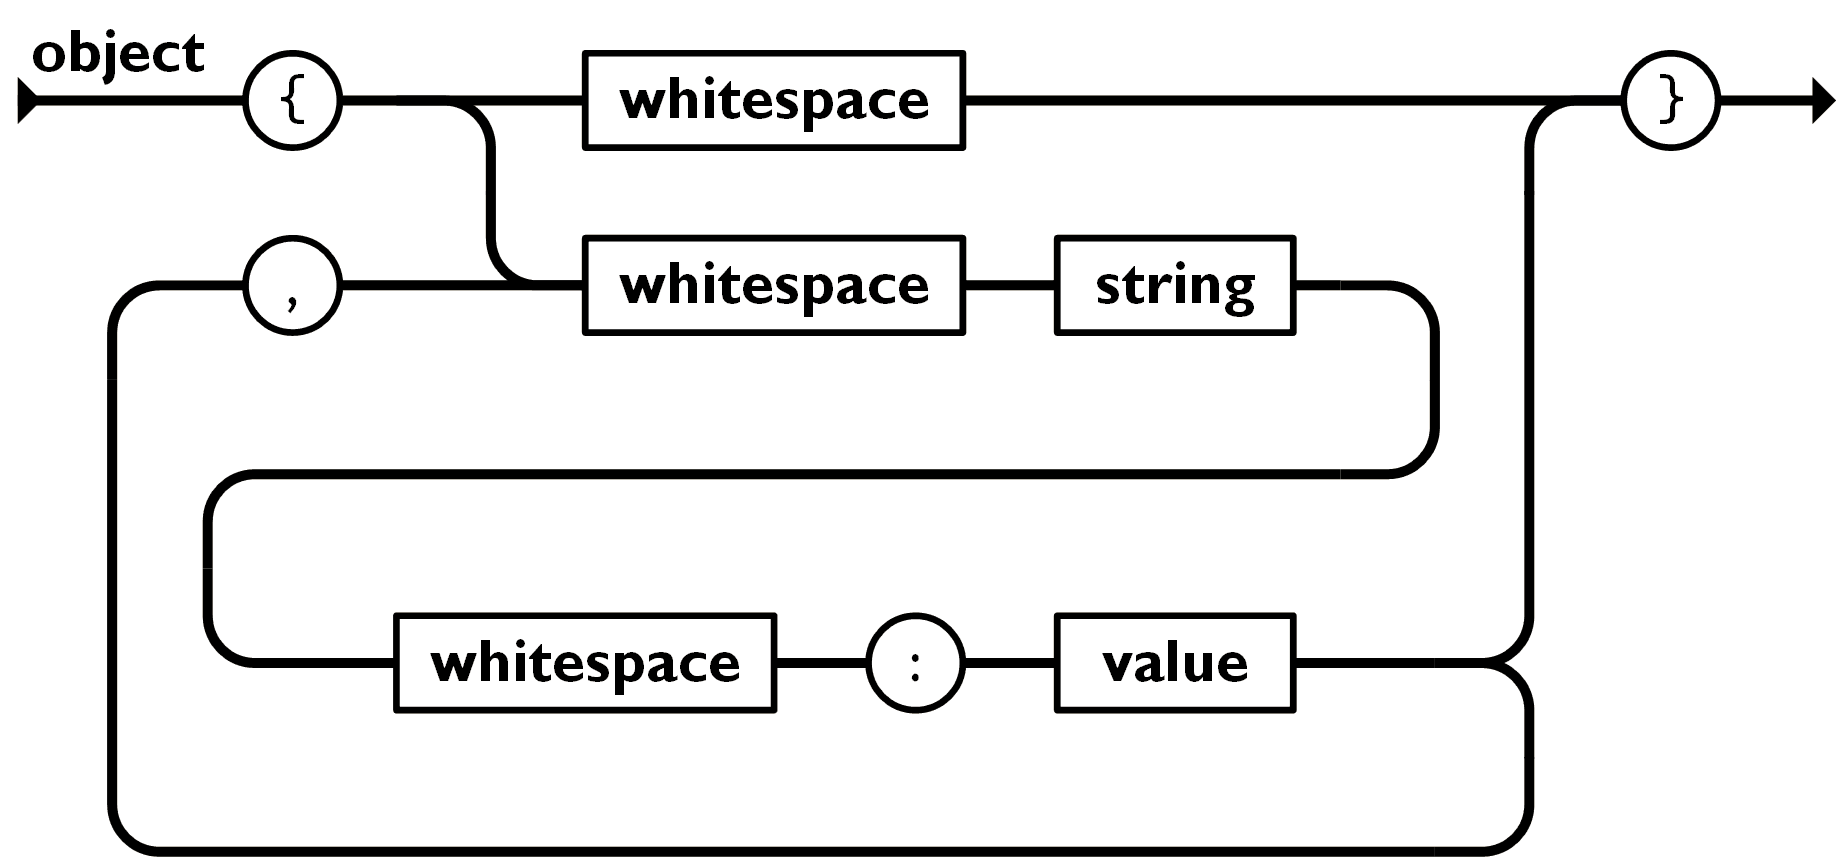
\includegraphics[scale=0.75]{jsonObject}
\caption[JSON Object Structuur]{De structuur van een JSON object. Bron: \url{www.json.org}}
    \label{fig:jsonObject}
\end{figure}

\begin{figure}[H]
    \centering
    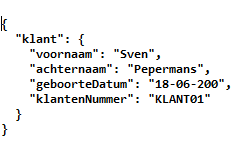
\includegraphics[scale=1.5]{objectEx}
    \caption[JSON Object]{Voorbeeld van een JSON object.}
    \label{fig:objectEx}
\end{figure}

Een tweede waarde zijn de arrays, dit zijn vierkante haken die geen of meerdere waarden omringen. Het bijzondere aan arrays is dat deze niet beperkt zijn tot een name/value paar en dus ook andere arrays kunnen bevatten en genest kunnen worden. Dit kan afgeleid worden uit figuur \ref{fig:jsonArray}. De array structuur wordt net zoals bij objecten geen beperkingen opgelegd, echter worden deze vooral gebruikt in situaties waar de ordening wel enig belang heeft. Figuur \ref{fig:arrayEx} is hier een duidelijk voorbeeld van.

\begin{figure}[H]
    \centering
    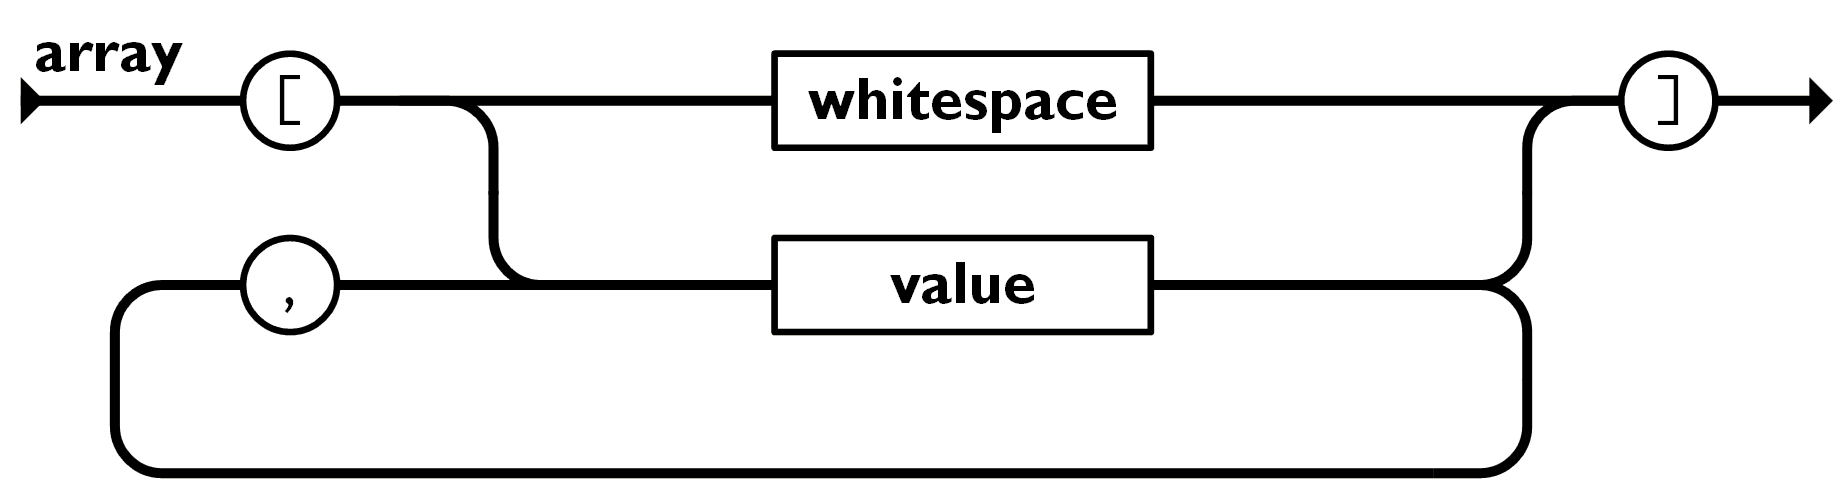
\includegraphics[scale=0.75]{jsonArray}
    \caption[JSON Array Structuur]{De structuur van een JSON array. Bron: \url{www.json.org}}
    \label{fig:jsonArray}
\end{figure}
\begin{figure}[H]
    \centering
    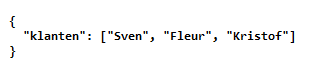
\includegraphics[scale=1.50]{arrayEx}
    \caption[JSON Array]{Een voorbeeld van een JSON Array.}
    \label{fig:arrayEx}
\end{figure}

Als volgt zijn er de nummers, een nummer kan gedefinieerd worden als een sequentie van decimale cijfers. Bij deze sequentie cijfers is er geen overbodige voorloopnul, een nummer kan wel voorafgegaan worden door een min-teken, als ook kan een nummer voorafgegaan worden door zowel een kleine als een grote e om een exponent aan te duiden dat  eventueel kan worden bijgestaan door een plus- of min-teken. Om te werken met kommagetallen wordt een decimaal punt gebruikt. Deze structuur is te zien in figuur \ref{fig:jsonNumber} en een voorbeeld hiervan in figuur \ref{fig:numberEx}.

\begin{figure}[H]
    \centering
    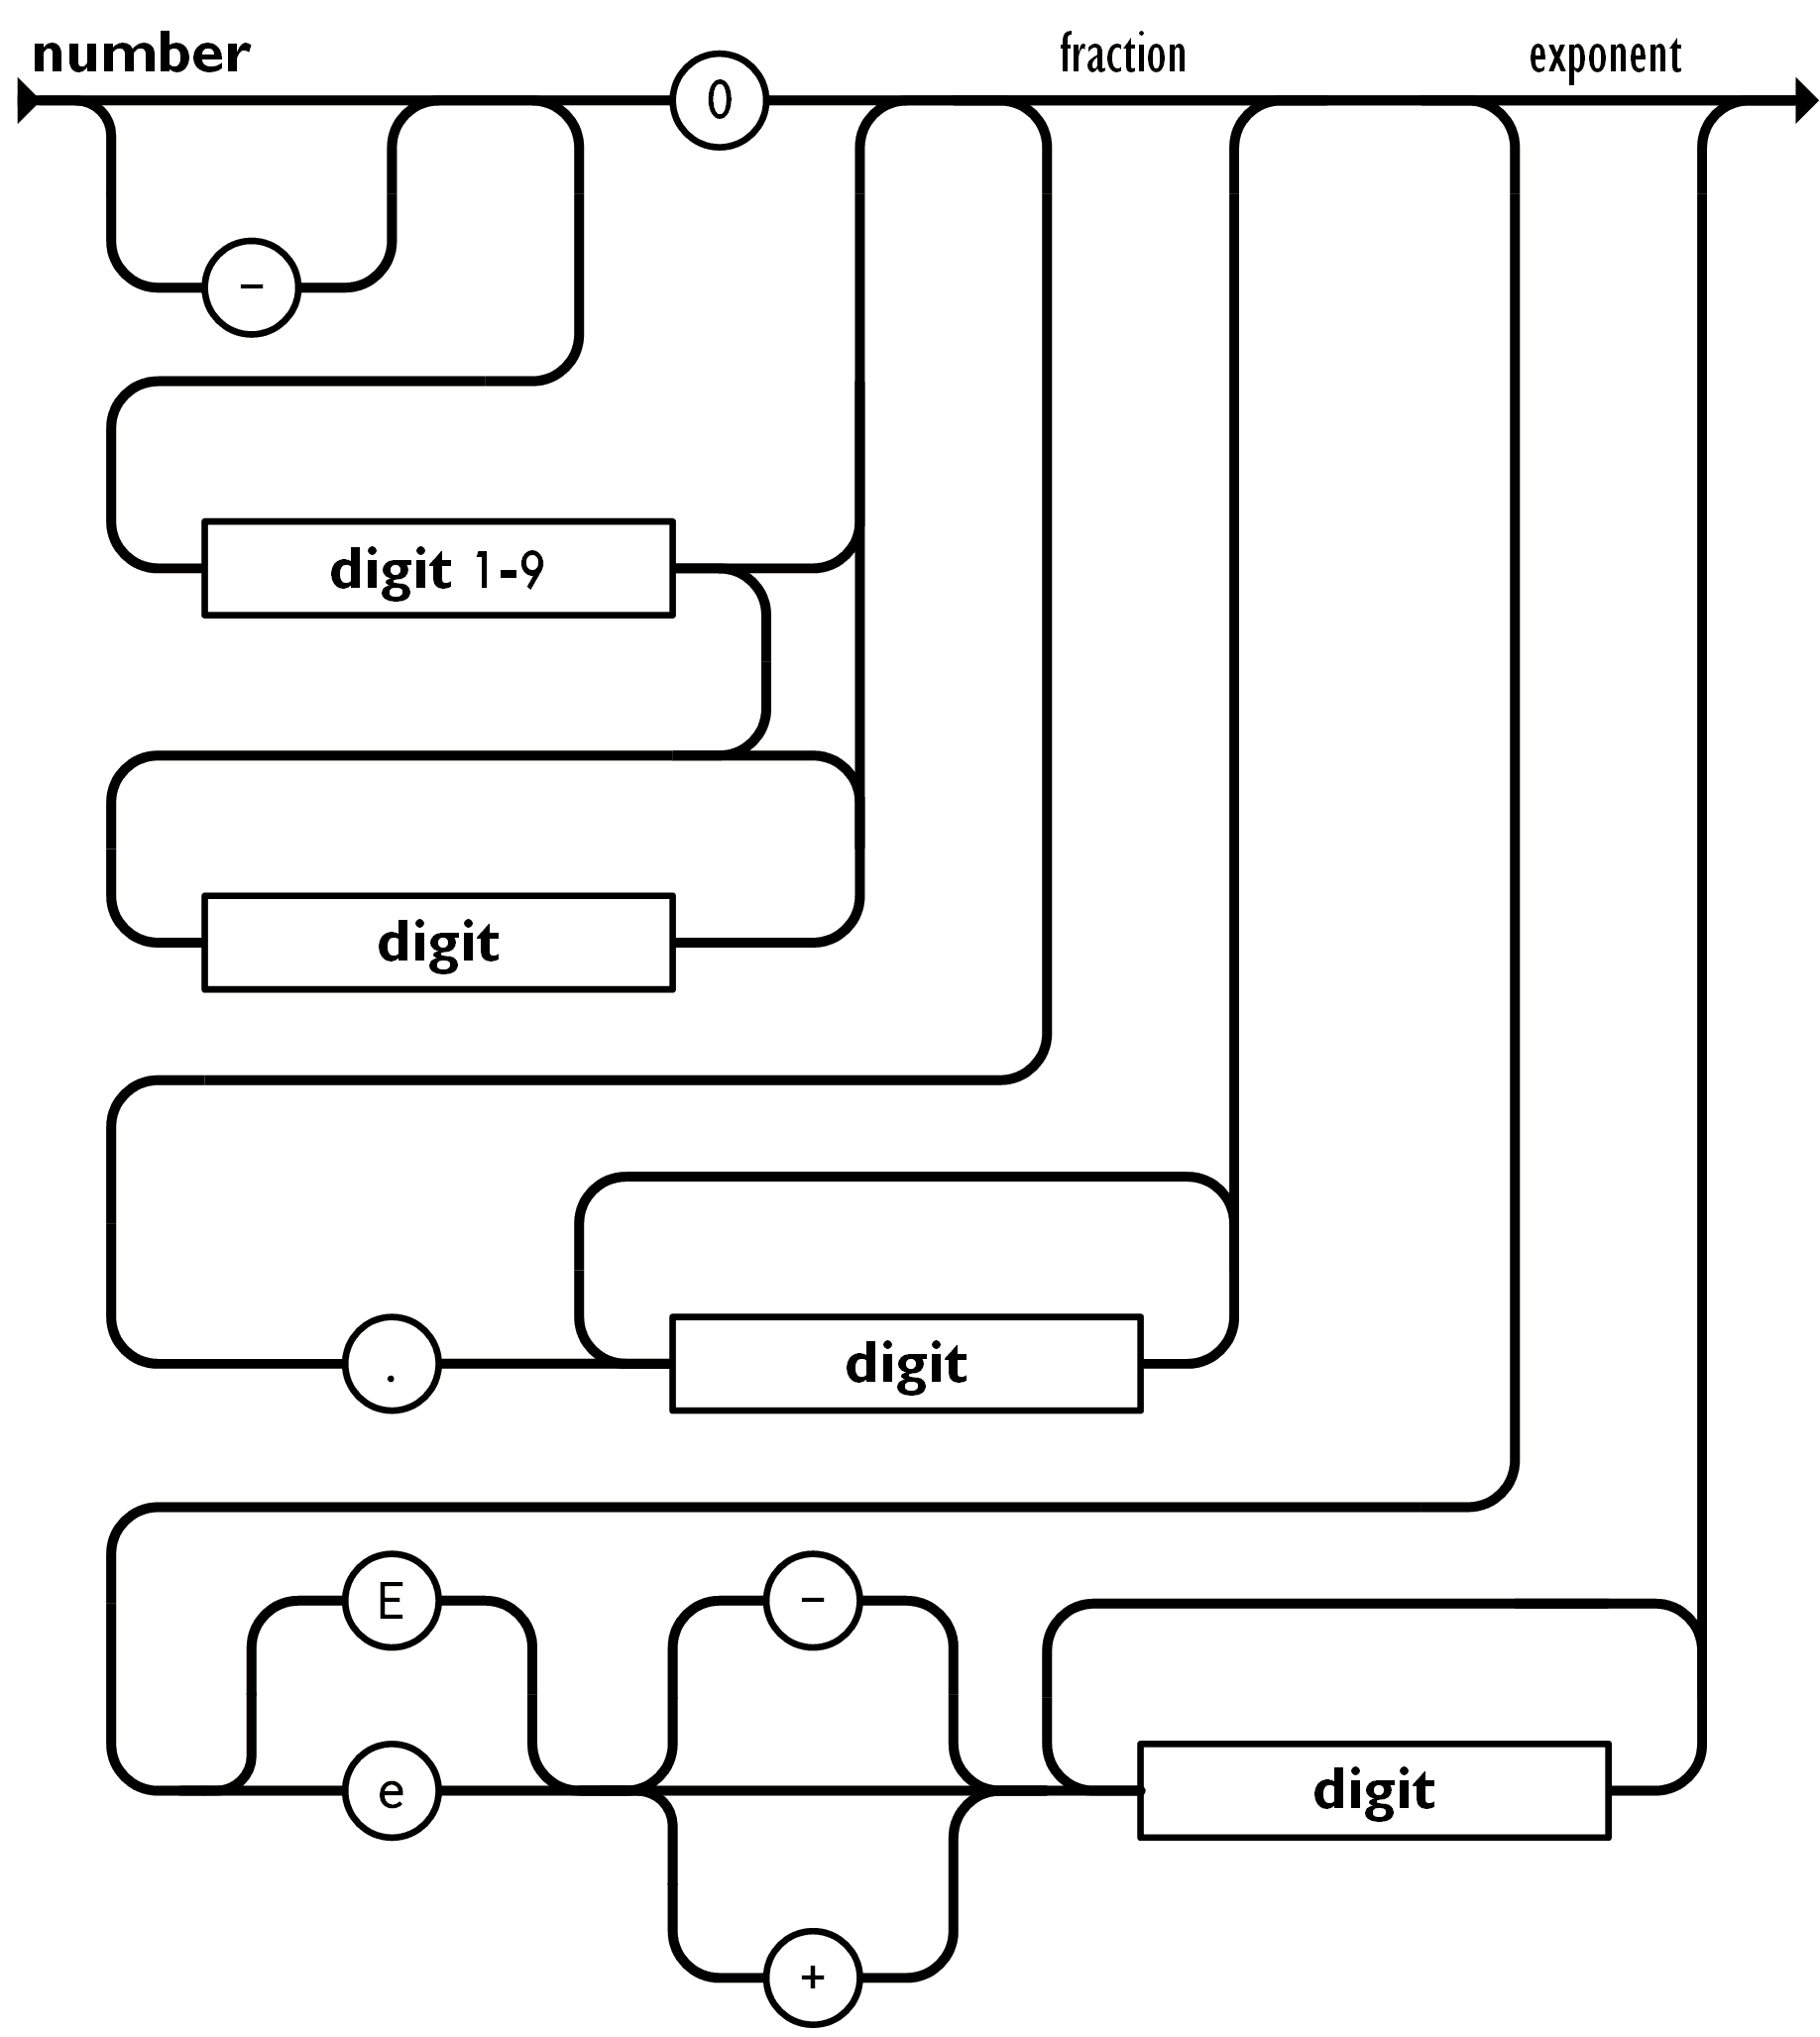
\includegraphics[scale=0.7]{jsonNumber}
    \caption[JSON Nummer Structuur]{De structuur van een JSON nummer. Bron: \url{www.json.org}}
    \label{fig:jsonNumber}
\end{figure}

\begin{figure}[H]
    \centering
    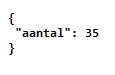
\includegraphics[scale=1.50]{numberEx}
    \caption[JSON Nummer]{Een voorbeeld van een JSON nummer.}
    \label{fig:numberEx}
\end{figure}

Tot slot zijn er de strings, deze representeren een tekst-waarde bestaande uit een sequentie van Unicode codepunten en zijn omringt door aanhalingstekens. Binnen deze aanhalingstekens zijn er echter enkele codepunten die niet gebruikt mogen worden, namelijk de karakters die moeten worden geëscaped. Dit zijn dan aanhalingstekens, backslash en de control karakters.
Voor sommige escape-reeksweergaven bestaande uit twee tekens bestaat er wel een representatie binnen de string, een representatie hiervan is te zien in \ref{fig:jsonString}.

Daarnaast kan ook elk codepunt weergegeven worden als een hexadecimale sequentie, waarvan de betekenis is vastgelegd in ISO/IEC 10646. Hexadecimale getallen kunnen zowel cijfers als kleine letters en hoofdletters van A tot F zijn.
De codepunten die zich bevinden in het Basic Multilingual Plane kunnen gerepresenteerd worden als een sequentie van zes karakters, namelijk een backslash gevolgd door een kleine letter u, en tot slot gevolgd door vier hexadecimale getallen die een codepunt encoderen. In figuur \ref{fig:jsonString} is de structuur van een string te zien.

\begin{figure}[H]
    \centering
    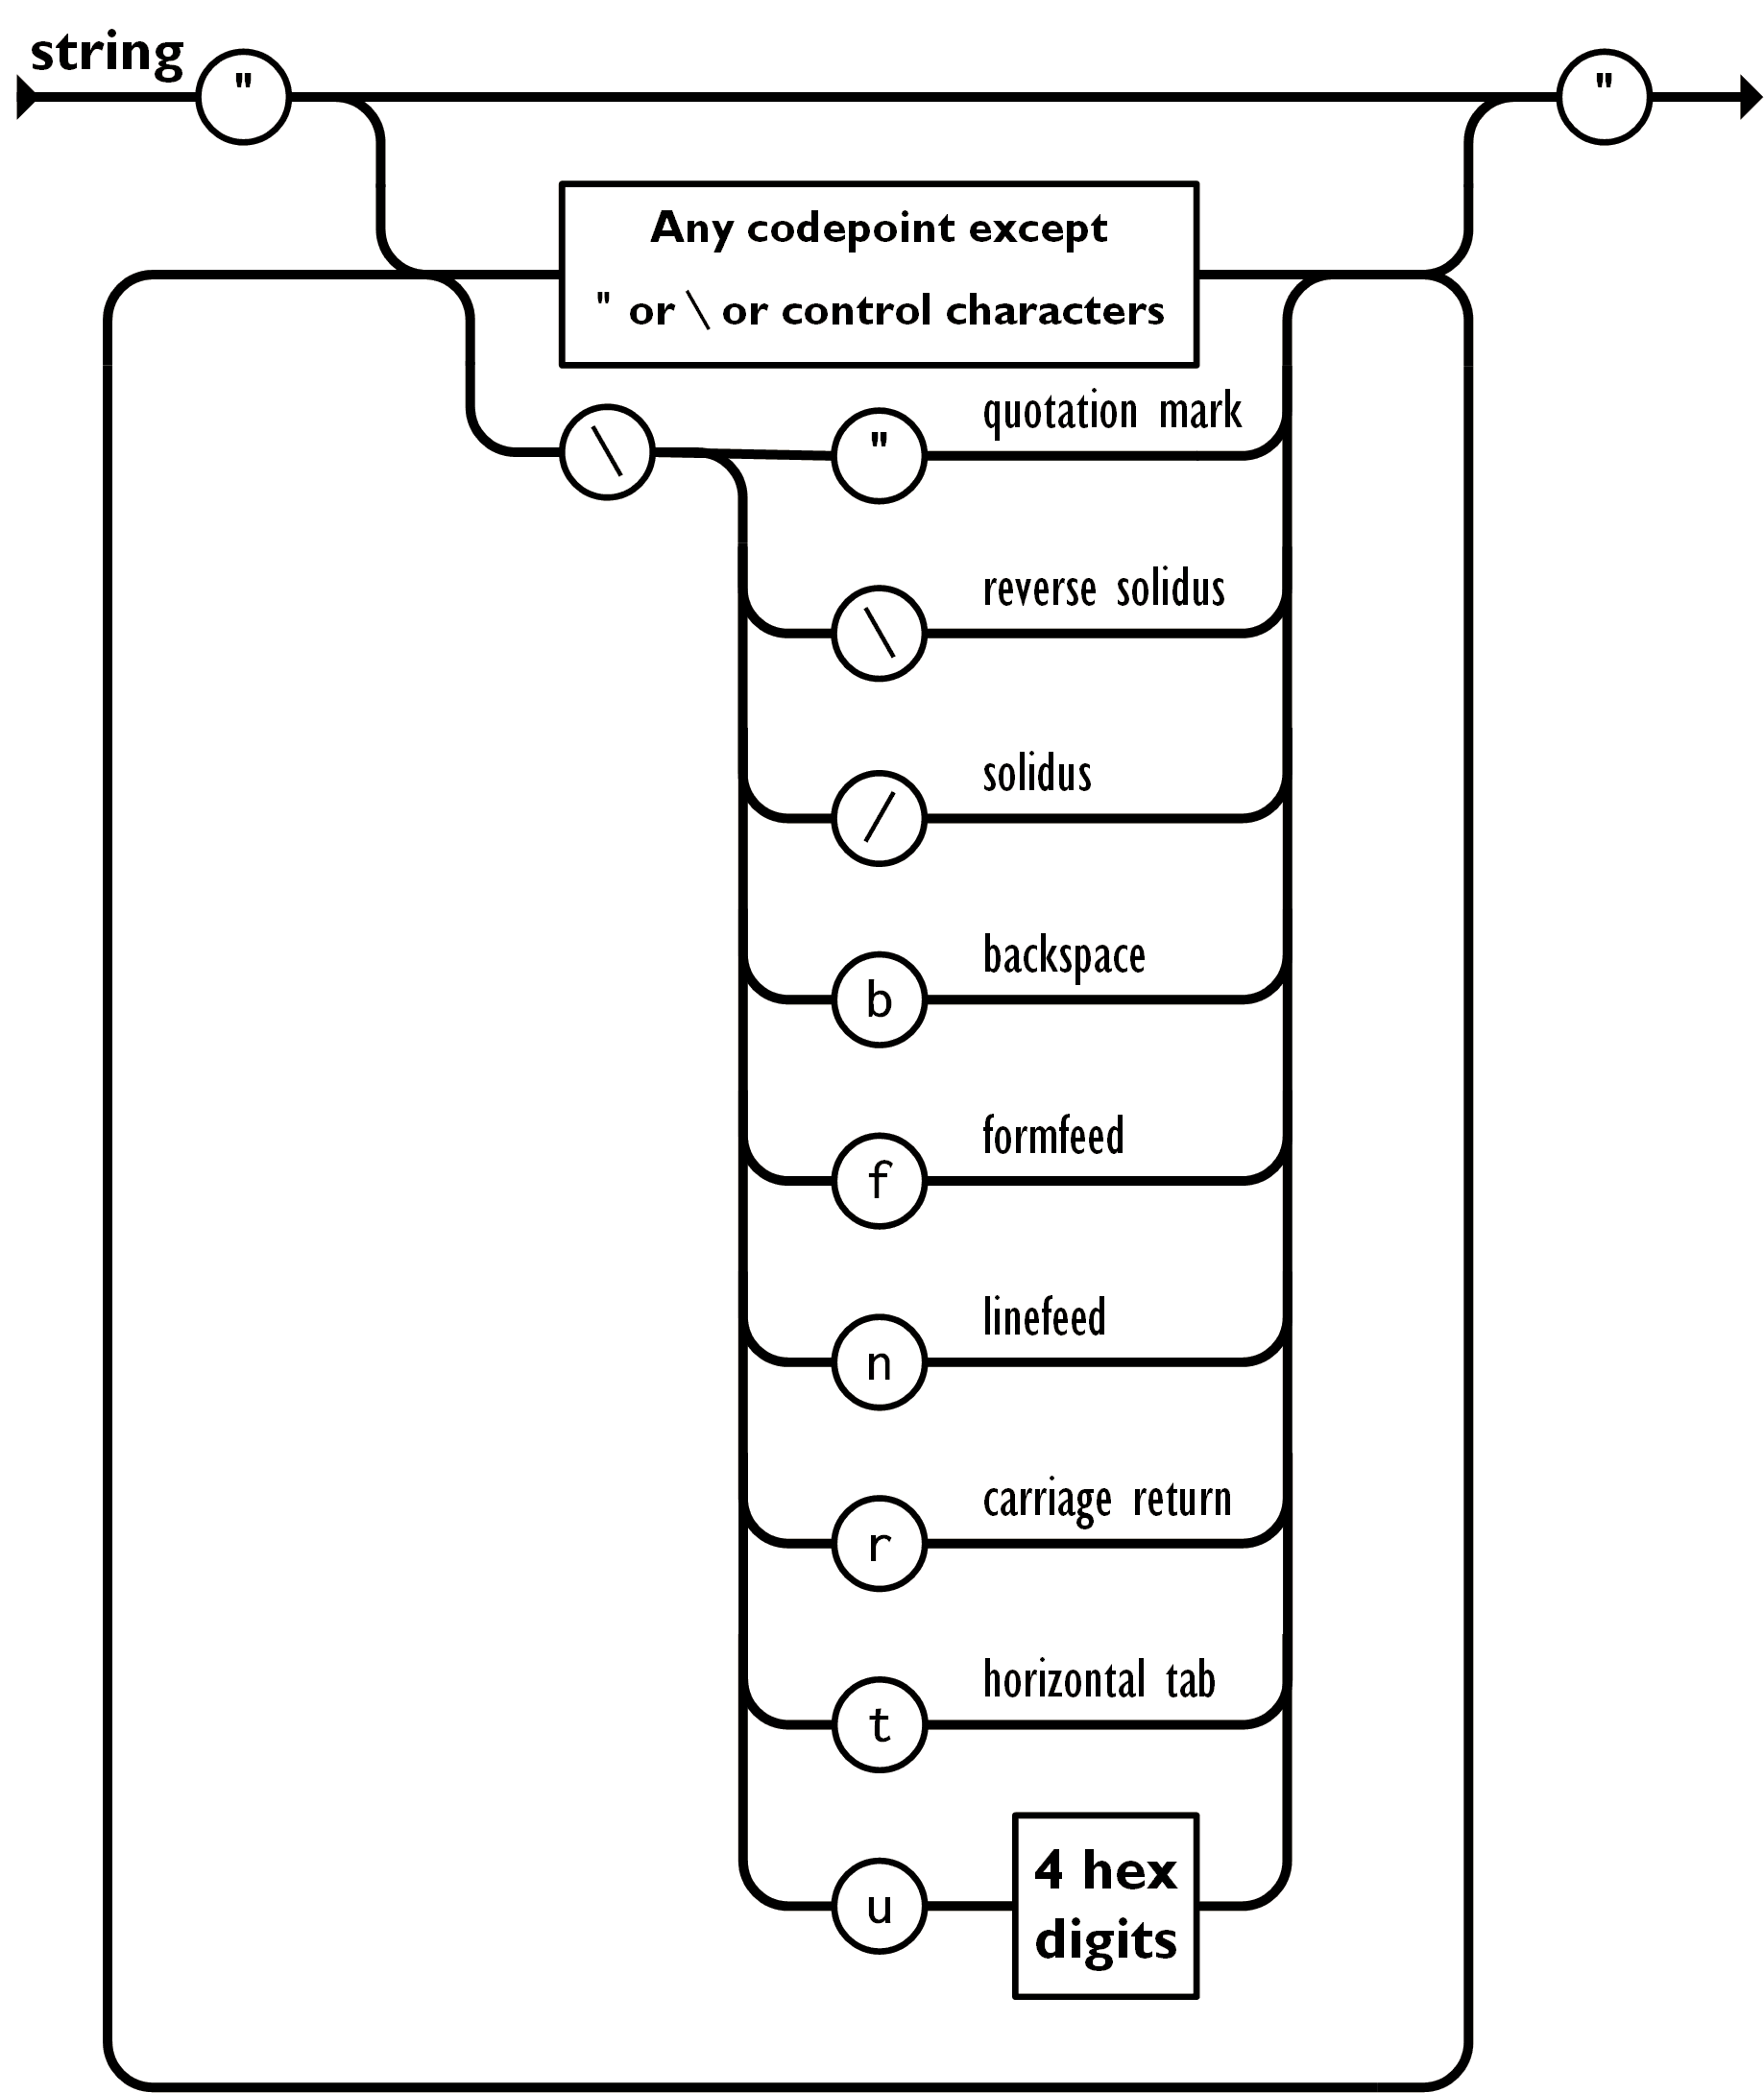
\includegraphics[scale=0.75]{jsonString}
    \caption[JSON String]{De structuur van een JSON string. Bron: \url{www.json.org}}
    \label{fig:jsonString}
\end{figure}


\section{RESTful API}
\label{sec:RESTful API}

Representational State Transfer (REST) is zoals beschreven door \textcite{Fielding2000} een architecturale stijl voor het ontwerpen van gedistribueerde hypermediasystemen.
Een Application Program Interface (API) is een lijst van regels of restricties die ervoor zorgen dat verschillende programma's met elkaar kunnen communiceren. \autocite{Hubspire}

De combinatie van REST en API is een RESTful API, wanneer een RESTful API gecalled wordt dan zal de server een representatie van de huidige staat van de gevraagde resource weergeven.

\subsection{Design principes}
\label{subsec:Design principes}

Om een API als RESTful te kunnen beschrijven moet deze voldoen aan zes design principes die hieronder zullen worden verduidelijkt aan de hand van \autocite{Long} en \autocite{Naeem2021}

\textbf{Client-Server}

Dit principe zegt dat zowel de client als de server apart moeten kunnen worden ontwikkeld en moeten los staan van elkaar. Op deze manier wordt de handelbaarheid en schaalbaarheid aanzienlijk verbetered aangezien de gebruikersinterface los staat van de gegevensopslag.


\textbf{Stateless}

Met stateless wordt bedoeld dat elke request die er naar de API gedaan wordt onafhankelijk is van elkaar, een request heeft dus geen resultaat nodig van een andere request om te kunnen verder gaan. Met andere woorden moet de server geen vorige requests en states opslaan wat de benaming 'Stateless' verklaard.


\textbf{Cacheable}

Een REST API moet de mogelijkheid hebben om data te cachen, dit is het opslaan van data in digitaal geheugen. Volgens het Cacheable principe moet data in een response al dien niet duidelijk gecategoriseerd worden als cacheable of non-cacheable. Indien een response cacheable is dan mag de cliënt cache deze data opslaan voor gelijkaardige requests in de toekomst te beantwoorden.

\textbf{Uniform interface}

Voor aan het client-server principe te voldoen is een uniforme interface nodig die autonome ontwikkeling van de applicatie mogelijk maakt zonder de acties, modellen en services te koppelen aan de API-laag. Door dit principe wordt de hele architectuur gestroomlijnd en wordt de visibiliteit van de communicatie verbeterd. Er zijn echter wel verschillende architecturale controles nodig die de performantie binnen de architectuur sturen om een uniforme interface te bereiken.

REST bevat vier interfacecontroles, namelijk: 

\begin{enumerate}
\item Identificatie van bronnen: Een Uniform Resource Locator (URL) identificeerd de online locatie van een resource.
\item Beheer van bronnen door middel van representatie: Bronnen worden weergegeven aan de hand van media types ~\autocite{N.Freed1996} zoals JSON en XML.
\item Zelfbeschrijvende communicatie: Een bericht bevat alle informatie die de ontvanger nodig heeft om de informatie te begrijpen. Er mag geen extra informatie in een aparte documentatie of apart bericht zitten. Deze zelfbeschrijvende communicatie gebeurd door het gebruik van de accept en content-type HTTP headers die de inhoud die verzonden of aangevraagd wordt beschrijft.
\item Hypermedia: Hypermedia is data dat verzonden wordt van de server naar de cliënt met informatie over wat de cliënt vervolgens kan doen. Hyper Text Markup Language (HTML) ~\autocite{W3schools} is hier een voorbeeld van.
\end{enumerate}
\textbf{Layered system}

De architectuur van een RESTful API bestaat uit verschillende lagen die door samen te werken een hiërarchie vormen die helpt bij het vormen van een flexibele, meer schaalbare applicatie. Dankzij het deze gelaagde structuur is de gevormde applicatie beter beveiligd, dit komt doordat componenten niet kunnen interageren buiten de eigen laag en de volgende laag. Daarnaast biedt het gedeelde caches aan die de schaalbaarheid verbeteren.

Deze gelaagde architectuur zorgt tot slot voor meer stabiliteit doordat het de componenten beperkt zodanig dat een component niet verder kan 'zien' als de laag waarmee het interageerd.

\textbf{Code on demand}

Het 'Code on demand' principe zorgt ervoor dat codering kan worden gecommuniceerd via de API voor gebruik binnen de applicatie. De definitie van een RESTful API maakt het mogelijk dat functionaliteit aan de cliënt-kant kan worden uitgebreid door codering zoals applets of scripts te downloaden en te implementeren. Dit stroomlijnt cliënts door het aantal functies te verminderen die vooraf moeten worden geïmplementeerd.

Naast statische resources zoals XML en JSON kan dus ook uitvoerbare code aangeleverd worden door de server.

\textbf{Resources}

Bij REST kan elk stuk informatie een resource zijn, dit kan van alles zijn zoals documenten, services, collecties van andere resources, afbeeldingen, en dergelijke. In sommige gevallen wordt “Everything as a resource”  een zevende principe van REST genoemd. 

\subsection{Hoe werkt een RESTful API?}
\label{subsec:Hoe werkt een RESTful API?}

Zoals eerder vermeld in subsectie \ref{subsec:Design principes} heeft elke resource een unieke URL, zo een URL wordt een request genoemd waarbij de gereturnde data gekend staat als een response. In een RESTful API worden deze requests of transacties in vier componenten verdeeld zoals uitgelegd in \autocite{Karine2020}.

\begin{itemize}
    \item \textbf{GET}: Deze request haalt een representatie van een resource op.
    \item \textbf{PUT}: Met PUT wordt een bestaande resource geupdatet.
    \item \textbf{POST}: Aan de hand van POST kunnen nieuwe resources en sub-resources aangemaakt worden.
    \item \textbf{DELETE}: De DELETE request gaat een reeds bestaande resource verwijderen.
\end{itemize}

\section{Protocol Buffers}
\label{sec:Protocol Buffers}

 In dit hoofdstuk zal Protocol Buffers verduidelijkt worden, dit is het dataformaat dat gebruikt zal worden bij de implementatie van gRPC. In dit onderzoek is Protocol Buffers de tegenhanger van JSON.

\subsection{Wat zijn protocol buffers?}
\label{subsec:Wat zijn protocol buffers?}

Protocol buffers (protobuf) zijn net zoals JSON een manier om data te verzenden of op te slaan in bestanden en is ontwikkeld door Google zoals beschreven door \textcite{Kurion2020}. Een voorbeeld van een protobuf is te zien in figuur \ref{fig:protobufEx}.

\begin{figure}[H]
    \centering
    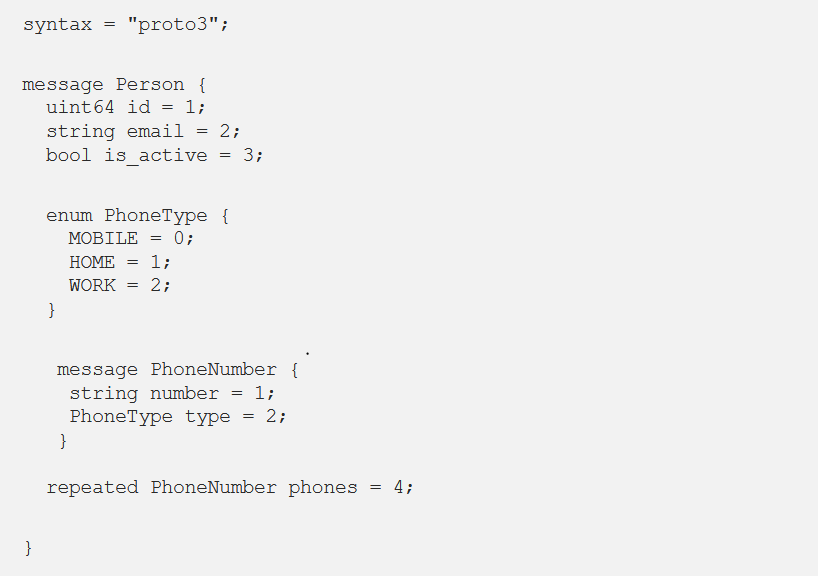
\includegraphics[scale=0.75]{protobufEx}
    \caption[Protocol Buffer .proto bestand]{Een voorbeeld van een .proto bestand. (Bron: \url{https://betterprogramming.pub/understanding-protocol-buffers-43c5bced0d47})}
    \label{fig:protobufEx}
\end{figure}

Formaten zoals JSON en XML zijn zeer flexibel maar zijn niet geoptimaliseerd voor het uitwisselen van data tussen meerdere microservices \autocite{Fowler2014} ongeacht het gebruikte platform. Protobuf is ontwikkeld met het oog op simpliciteit en performantie, om specifiek te zijn was het ontwikkeld om kleiner en sneller te zijn dan XML.

Protobuf onderscheidt zich van andere dataformaten door vele verantwoordelijkheden te verwijderen die normaal door het dataformaat aangepakt worden. Hierdoor gaat protobuf zich vooral focussen op het zo snel mogelijk serialiseren en deserialiseren van data. Daarnaast is een tweede optimalisatie de bandbreedte die gebruikt wordt door het zo klein mogelijk maken van de data die verzonden wordt.

Natuurlijk kan protobufs niet alleen voordelen hebben, een objectief nadeel dat protobuf heeft is dat het minder leesbaar is in vergelijking met JSON en XML.


\subsection{Kerneigenschappen}
\label{subsec:Kerneigenschappen}

\textbf{Binair formaat}

Protobuf is een binair dataformaat, dit betekend dat de verzonden data omgezet wordt naar ééntjes en nulletjes. Deze eigenschap zorgt voor een verbetering van de transmissiesnelheid doordat het dataformaat minder bandbreedte en ruimte inpakt. Tot slot zorgt de omzetting van string naar binair formaat ook voor compressie, hierdoor zal het CPU gebruik ook lager zijn.

\textbf{Splitsing van context en data}

Zoals in \ref{fig:JSONsEx} te zien is maakt een formaat zoals JSON gebruik van key-value paren waar de data en de context in éénzelfde bestand zitten wat ook meer ruimte in beslag neemt. Bij protobuf is dit anders, hier worden data en context opgesplitst in een configuratiebestand ook wel gekend als een .proto bestand, waarin de message wordt gedefinieerd, zie figuur \ref{fig:protobufEx}, en geëncodeerde data die verzonden wordt aan de hand van het configuratiebestand.

\begin{figure}[H]
    \centering
    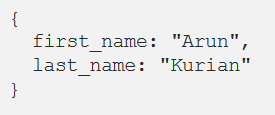
\includegraphics[scale=0.75]{JSONsEx}
    \caption[Simpel JSON key-value voorbeeld]{Een simpel voorbeeld van een key-value JSON bestand. (Bron: \url{https://betterprogramming.pub/understanding-protocol-buffers-43c5bced0d47})}
    \label{fig:JSONsEx}
\end{figure}


\subsection{Message formaat}
\label{subsec:Message formaat}

Zoals hierboven vermeld is het configuratiebestand de plaats waarin de context gedefinieerd wordt, met andere woorden wordt hier de structuur van een bepaald object bepaald. Deze structuur wordt als gedeclareerd door het “message” woord gevolgd door een zelfgekozen naam voor de message. Net zoals bij JSON worden de velden gedeclareerd binnen de accolades, deze velden kunnen elk in vier delen opgedeeld worden, namelijk veldregels, veldtypes, veldnamen en veldnummers \autocite{Google2020}.

\textbf{Veldregels}

In proto3 wordt enkel nog de “repeated” regel gebruikt, deze regel zegt dat de message dit veld meerdere keren mag bevatten met verschillende waarden. Met andere woorden, duid dit op een array van een bepaald veldtype.

In proto2 waren er ook de required en optional regels. Required zorgt ervoor dat een message een bepaald veld exact één keer bevat en de optional regel zorgt ervoor dat een message een veld nul of één keer kan bevatten.

\textbf{Veldtypes}

Het field type is het datatype van een field, dit zijn er vier:

\begin{itemize}
    \item \textbf{Scalaire types}: Dit zijn de traditionele types zoals strings, integers, booleans, ...
    \item \textbf{Enum}: Binnen een message is het mogelijk om een attribuut te hebben dat enkel één van een aantal vooraf bepaalde waarden mag hebben.
    \item \textbf{Message types}: Net zoals bij andere dataformaten is het mogelijk dat een message andere messages als attribuut bevat.
\end{itemize}

\textbf{Veldnamen}

Veldnamen moeten volledig in kleine letters zijn en indien ze uit meerdere woorden bestaan moeten deze opgesplitst worden door een underscore. In tegenstelling tot JSON wordt hier dus geen camelcasing gebruikt. Deze conventies zijn vastgelegd omdat dit ook de conventies zijn die gevolgd worden door de Protoc compiler die code gaat genereren op basis van het .proto bestand.

\textbf{Veldnummer}

Elk veld heeft een uniek nummer, deze nummers worden gebruikt om de velden te identificeren in het binaire formaat. Als gevolg mogen deze niet veranderd worden eens het message type reeds gebruikt is.









